\documentclass{article}
\usepackage{listings}

% Language setting
% Replace `english' with e.g. `spanish' to change the document language
\usepackage[english]{babel}

% Set page size and margins
% Replace `letterpaper' with`a4paper' for UK/EU standard size
\usepackage[letterpaper,top=2cm,bottom=2cm,left=3cm,right=3cm,marginparwidth=1.75cm]{geometry}

% Useful packages
\usepackage{amsmath}
\usepackage{graphicx}
\usepackage[colorlinks=true, allcolors=blue]{hyperref}

\title{Lab 2}
\author{Rick, Shae, and Owen}

\begin{document}
\maketitle

\section{Code Base}

The code base for Lab 2 is \href{https://github.com/owenbean400/COS470Lab2/tree/master}{https://github.com/owenbean400/COS470Lab2/tree/master}. To run the program step 2, type \verb|python3 main.py| in the command line. To run the extra credit step 3, install wordcloud by typing \verb|python3 -m pip install wordcloud| in the command line. Run the \verb|words_surrounding_numbers.py| in the command line.

\section{Word Cloud Step 3}

Analyzing the top 20 words, the most common word that came either before or after a number was "Covid". This is because a lot of the articles had Covid 19. The second most common was "least". This is because a lot of number statistics came after the word "least". The third most common word either before or after a number is "than". This is because "than" was used to compare a quantify number. For example, a common phrase was "More than $<$Number$>$  $<$Noun$>$".

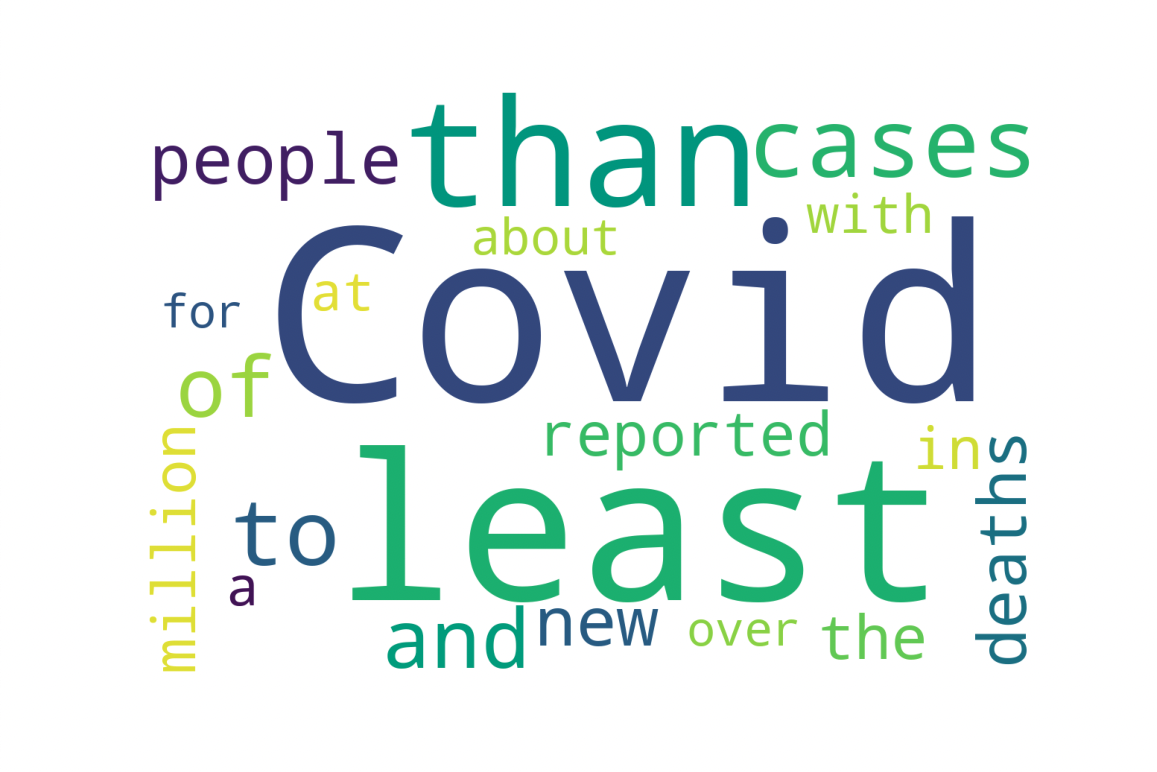
\includegraphics[width=\textwidth]{wordcloud.png}

\section{Output from Step 2}

\lstinputlisting[language={},breaklines=true,basicstyle=\small]{results.txt}

\end{document}